% Options for packages loaded elsewhere
\PassOptionsToPackage{unicode}{hyperref}
\PassOptionsToPackage{hyphens}{url}
\PassOptionsToPackage{dvipsnames,svgnames,x11names}{xcolor}
%
\documentclass[
  letterpaper,
  DIV=11,
  numbers=noendperiod]{scrartcl}

\usepackage{amsmath,amssymb}
\usepackage{iftex}
\ifPDFTeX
  \usepackage[T1]{fontenc}
  \usepackage[utf8]{inputenc}
  \usepackage{textcomp} % provide euro and other symbols
\else % if luatex or xetex
  \usepackage{unicode-math}
  \defaultfontfeatures{Scale=MatchLowercase}
  \defaultfontfeatures[\rmfamily]{Ligatures=TeX,Scale=1}
\fi
\usepackage{lmodern}
\ifPDFTeX\else  
    % xetex/luatex font selection
\fi
% Use upquote if available, for straight quotes in verbatim environments
\IfFileExists{upquote.sty}{\usepackage{upquote}}{}
\IfFileExists{microtype.sty}{% use microtype if available
  \usepackage[]{microtype}
  \UseMicrotypeSet[protrusion]{basicmath} % disable protrusion for tt fonts
}{}
\makeatletter
\@ifundefined{KOMAClassName}{% if non-KOMA class
  \IfFileExists{parskip.sty}{%
    \usepackage{parskip}
  }{% else
    \setlength{\parindent}{0pt}
    \setlength{\parskip}{6pt plus 2pt minus 1pt}}
}{% if KOMA class
  \KOMAoptions{parskip=half}}
\makeatother
\usepackage{xcolor}
\setlength{\emergencystretch}{3em} % prevent overfull lines
\setcounter{secnumdepth}{-\maxdimen} % remove section numbering
% Make \paragraph and \subparagraph free-standing
\ifx\paragraph\undefined\else
  \let\oldparagraph\paragraph
  \renewcommand{\paragraph}[1]{\oldparagraph{#1}\mbox{}}
\fi
\ifx\subparagraph\undefined\else
  \let\oldsubparagraph\subparagraph
  \renewcommand{\subparagraph}[1]{\oldsubparagraph{#1}\mbox{}}
\fi


\providecommand{\tightlist}{%
  \setlength{\itemsep}{0pt}\setlength{\parskip}{0pt}}\usepackage{longtable,booktabs,array}
\usepackage{calc} % for calculating minipage widths
% Correct order of tables after \paragraph or \subparagraph
\usepackage{etoolbox}
\makeatletter
\patchcmd\longtable{\par}{\if@noskipsec\mbox{}\fi\par}{}{}
\makeatother
% Allow footnotes in longtable head/foot
\IfFileExists{footnotehyper.sty}{\usepackage{footnotehyper}}{\usepackage{footnote}}
\makesavenoteenv{longtable}
\usepackage{graphicx}
\makeatletter
\def\maxwidth{\ifdim\Gin@nat@width>\linewidth\linewidth\else\Gin@nat@width\fi}
\def\maxheight{\ifdim\Gin@nat@height>\textheight\textheight\else\Gin@nat@height\fi}
\makeatother
% Scale images if necessary, so that they will not overflow the page
% margins by default, and it is still possible to overwrite the defaults
% using explicit options in \includegraphics[width, height, ...]{}
\setkeys{Gin}{width=\maxwidth,height=\maxheight,keepaspectratio}
% Set default figure placement to htbp
\makeatletter
\def\fps@figure{htbp}
\makeatother

\usepackage{fontspec}
\usepackage{multirow}
\usepackage{multicol}
\usepackage{colortbl}
\usepackage{hhline}
\newlength\Oldarrayrulewidth
\newlength\Oldtabcolsep
\usepackage{longtable}
\usepackage{array}
\usepackage{hyperref}
\usepackage{float}
\usepackage{wrapfig}
\KOMAoption{captions}{tableheading}
\makeatletter
\makeatother
\makeatletter
\makeatother
\makeatletter
\@ifpackageloaded{caption}{}{\usepackage{caption}}
\AtBeginDocument{%
\ifdefined\contentsname
  \renewcommand*\contentsname{Table of contents}
\else
  \newcommand\contentsname{Table of contents}
\fi
\ifdefined\listfigurename
  \renewcommand*\listfigurename{List of Figures}
\else
  \newcommand\listfigurename{List of Figures}
\fi
\ifdefined\listtablename
  \renewcommand*\listtablename{List of Tables}
\else
  \newcommand\listtablename{List of Tables}
\fi
\ifdefined\figurename
  \renewcommand*\figurename{Figure}
\else
  \newcommand\figurename{Figure}
\fi
\ifdefined\tablename
  \renewcommand*\tablename{Table}
\else
  \newcommand\tablename{Table}
\fi
}
\@ifpackageloaded{float}{}{\usepackage{float}}
\floatstyle{ruled}
\@ifundefined{c@chapter}{\newfloat{codelisting}{h}{lop}}{\newfloat{codelisting}{h}{lop}[chapter]}
\floatname{codelisting}{Listing}
\newcommand*\listoflistings{\listof{codelisting}{List of Listings}}
\makeatother
\makeatletter
\@ifpackageloaded{caption}{}{\usepackage{caption}}
\@ifpackageloaded{subcaption}{}{\usepackage{subcaption}}
\makeatother
\makeatletter
\@ifpackageloaded{tcolorbox}{}{\usepackage[skins,breakable]{tcolorbox}}
\makeatother
\makeatletter
\@ifundefined{shadecolor}{\definecolor{shadecolor}{rgb}{.97, .97, .97}}
\makeatother
\makeatletter
\makeatother
\makeatletter
\makeatother
\ifLuaTeX
  \usepackage{selnolig}  % disable illegal ligatures
\fi
\IfFileExists{bookmark.sty}{\usepackage{bookmark}}{\usepackage{hyperref}}
\IfFileExists{xurl.sty}{\usepackage{xurl}}{} % add URL line breaks if available
\urlstyle{same} % disable monospaced font for URLs
\hypersetup{
  pdftitle={SC21 Length data explore for climate indicators},
  colorlinks=true,
  linkcolor={blue},
  filecolor={Maroon},
  citecolor={Blue},
  urlcolor={Blue},
  pdfcreator={LaTeX via pandoc}}

\title{SC21 Length data explore for climate indicators}
\author{}
\date{}

\begin{document}
\maketitle
\ifdefined\Shaded\renewenvironment{Shaded}{\begin{tcolorbox}[breakable, boxrule=0pt, enhanced, frame hidden, sharp corners, interior hidden, borderline west={3pt}{0pt}{shadecolor}]}{\end{tcolorbox}}\fi

\hypertarget{exploration-of-wcpfc-longline-length-frequency-data}{%
\subsection{Exploration of WCPFC longline length frequency
data}\label{exploration-of-wcpfc-longline-length-frequency-data}}

This document extracts length frequency data from SPC databases to
explore it in preparation for further analysis and potential use in
SPC's upcoming climate indicators report. Here, we focus on the longline
data given the complexity and issues associated with the use and
handling of purse seine length frequency data.

\hypertarget{database-extract}{%
\subsection{Database extract}\label{database-extract}}

Below, is the database extract from the updated fishmaster SPC database.

This data is then cleaned by the following filtering steps:

\begin{itemize}
\item
  WCPFC convention area
\item
  Longline gear only
\item
  BET and YFT only
\end{itemize}

\hypertarget{exploratory-plots}{%
\subsection{Exploratory plots}\label{exploratory-plots}}

Note that length data is collected in 2cm size bins.

\begin{figure}

{\centering 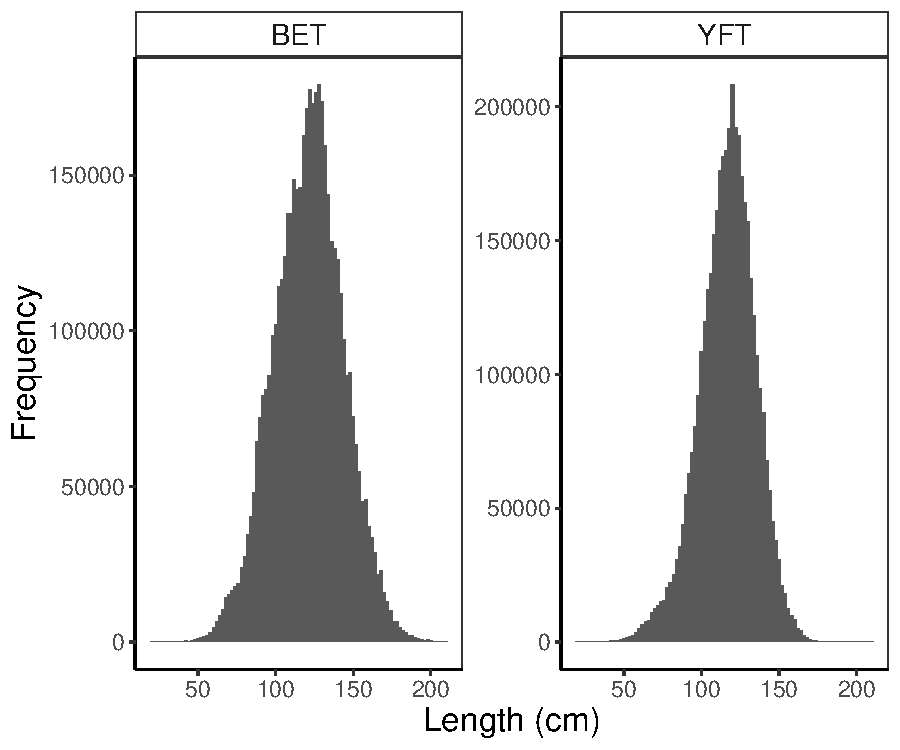
\includegraphics{length_data_explore_files/figure-pdf/raw_len_by_spp-1.pdf}

}

\caption{Raw length frequency data by species.}

\end{figure}

\begin{figure}

{\centering 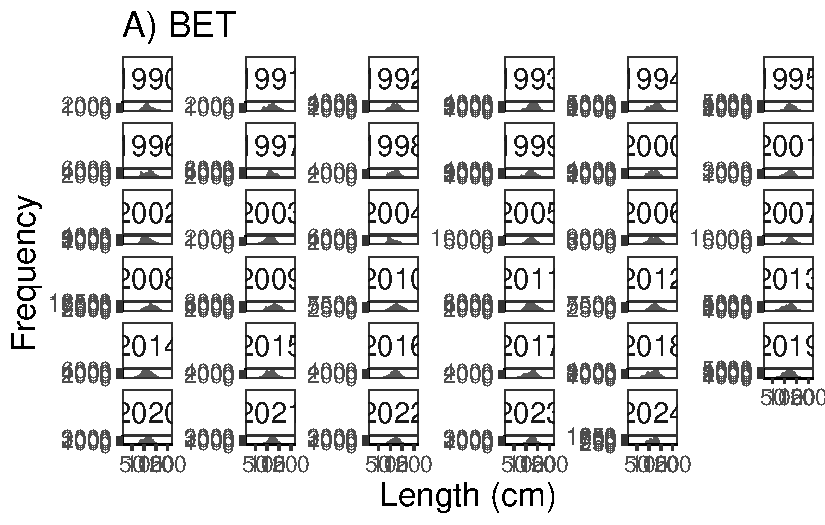
\includegraphics{length_data_explore_files/figure-pdf/raw_len_by_yr-1.pdf}

}

\caption{Raw length frequency data by year. A) BET, B) YFT.}

\end{figure}

\begin{figure}

{\centering 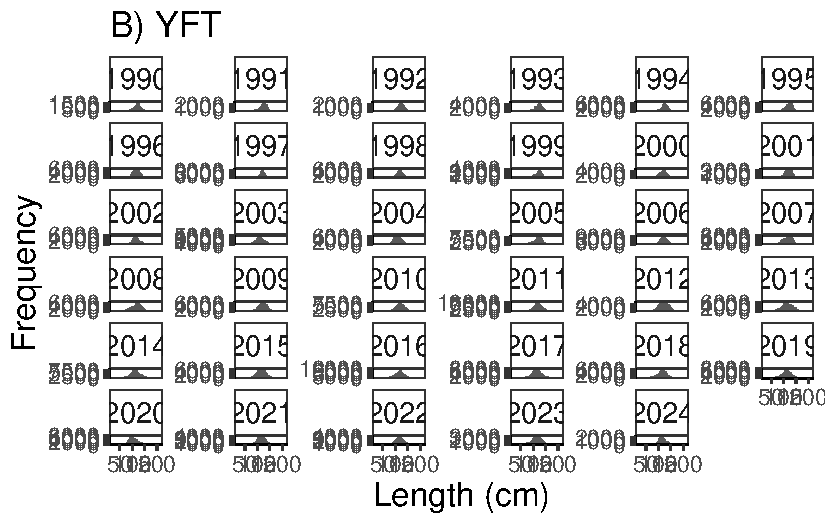
\includegraphics{length_data_explore_files/figure-pdf/raw_len_by_yr-2.pdf}

}

\caption{Raw length frequency data by year. A) BET, B) YFT.}

\end{figure}

\global\setlength{\Oldarrayrulewidth}{\arrayrulewidth}

\global\setlength{\Oldtabcolsep}{\tabcolsep}

\setlength{\tabcolsep}{0pt}

\renewcommand*{\arraystretch}{1.5}



\providecommand{\ascline}[3]{\noalign{\global\arrayrulewidth #1}\arrayrulecolor[HTML]{#2}\cline{#3}}

\begin{longtable}[c]{|p{0.93in}|p{3.87in}|p{0.96in}}
\caption{Description of length sampling programs and total sample sizes.}\tabularnewline




\ascline{1.5pt}{666666}{1-3}

\multicolumn{1}{>{\raggedright}m{\dimexpr 0.93in+0\tabcolsep}}{\textcolor[HTML]{000000}{\fontsize{11}{11}\selectfont{\textbf{Origin\ ID}}}} & \multicolumn{1}{>{\raggedright}m{\dimexpr 3.87in+0\tabcolsep}}{\textcolor[HTML]{000000}{\fontsize{11}{11}\selectfont{\textbf{Sampling\ program}}}} & \multicolumn{1}{>{\raggedleft}m{\dimexpr 0.96in+0\tabcolsep}}{\textcolor[HTML]{000000}{\fontsize{11}{11}\selectfont{\textbf{Sample\ n}}}} \\

\ascline{1.5pt}{666666}{1-3}\endfirsthead 

\ascline{1.5pt}{666666}{1-3}

\multicolumn{1}{>{\raggedright}m{\dimexpr 0.93in+0\tabcolsep}}{\textcolor[HTML]{000000}{\fontsize{11}{11}\selectfont{\textbf{Origin\ ID}}}} & \multicolumn{1}{>{\raggedright}m{\dimexpr 3.87in+0\tabcolsep}}{\textcolor[HTML]{000000}{\fontsize{11}{11}\selectfont{\textbf{Sampling\ program}}}} & \multicolumn{1}{>{\raggedleft}m{\dimexpr 0.96in+0\tabcolsep}}{\textcolor[HTML]{000000}{\fontsize{11}{11}\selectfont{\textbf{Sample\ n}}}} \\

\ascline{1.5pt}{666666}{1-3}\endhead



\multicolumn{1}{>{\raggedright}m{\dimexpr 0.93in+0\tabcolsep}}{\textcolor[HTML]{000000}{\fontsize{11}{11}\selectfont{AUOB}}} & \multicolumn{1}{>{\raggedright}m{\dimexpr 3.87in+0\tabcolsep}}{\textcolor[HTML]{000000}{\fontsize{11}{11}\selectfont{AFMA\ (AFZ)\ Observer\ Data}}} & \multicolumn{1}{>{\raggedleft}m{\dimexpr 0.96in+0\tabcolsep}}{\textcolor[HTML]{000000}{\fontsize{11}{11}\selectfont{103,215}}} \\

\ascline{0.75pt}{666666}{1-3}



\multicolumn{1}{>{\raggedright}m{\dimexpr 0.93in+0\tabcolsep}}{\textcolor[HTML]{000000}{\fontsize{11}{11}\selectfont{CKOB}}} & \multicolumn{1}{>{\raggedright}m{\dimexpr 3.87in+0\tabcolsep}}{\textcolor[HTML]{000000}{\fontsize{11}{11}\selectfont{Cook\ Islands\ Observer\ Programme}}} & \multicolumn{1}{>{\raggedleft}m{\dimexpr 0.96in+0\tabcolsep}}{\textcolor[HTML]{000000}{\fontsize{11}{11}\selectfont{40,638}}} \\

\ascline{0.75pt}{666666}{1-3}



\multicolumn{1}{>{\raggedright}m{\dimexpr 0.93in+0\tabcolsep}}{\textcolor[HTML]{000000}{\fontsize{11}{11}\selectfont{CS}}} & \multicolumn{1}{>{\raggedright}m{\dimexpr 3.87in+0\tabcolsep}}{\textcolor[HTML]{000000}{\fontsize{11}{11}\selectfont{Coral\ Sea\ Tagging}}} & \multicolumn{1}{>{\raggedleft}m{\dimexpr 0.96in+0\tabcolsep}}{\textcolor[HTML]{000000}{\fontsize{11}{11}\selectfont{974}}} \\

\ascline{0.75pt}{666666}{1-3}



\multicolumn{1}{>{\raggedright}m{\dimexpr 0.93in+0\tabcolsep}}{\textcolor[HTML]{000000}{\fontsize{11}{11}\selectfont{FJCT}}} & \multicolumn{1}{>{\raggedright}m{\dimexpr 3.87in+0\tabcolsep}}{\textcolor[HTML]{000000}{\fontsize{11}{11}\selectfont{Fiji\ In-country\ Tagging}}} & \multicolumn{1}{>{\raggedleft}m{\dimexpr 0.96in+0\tabcolsep}}{\textcolor[HTML]{000000}{\fontsize{11}{11}\selectfont{4}}} \\

\ascline{0.75pt}{666666}{1-3}



\multicolumn{1}{>{\raggedright}m{\dimexpr 0.93in+0\tabcolsep}}{\textcolor[HTML]{000000}{\fontsize{11}{11}\selectfont{FJOB}}} & \multicolumn{1}{>{\raggedright}m{\dimexpr 3.87in+0\tabcolsep}}{\textcolor[HTML]{000000}{\fontsize{11}{11}\selectfont{Fiji\ Observer\ Programme}}} & \multicolumn{1}{>{\raggedleft}m{\dimexpr 0.96in+0\tabcolsep}}{\textcolor[HTML]{000000}{\fontsize{11}{11}\selectfont{257,440}}} \\

\ascline{0.75pt}{666666}{1-3}



\multicolumn{1}{>{\raggedright}m{\dimexpr 0.93in+0\tabcolsep}}{\textcolor[HTML]{000000}{\fontsize{11}{11}\selectfont{FMOB}}} & \multicolumn{1}{>{\raggedright}m{\dimexpr 3.87in+0\tabcolsep}}{\textcolor[HTML]{000000}{\fontsize{11}{11}\selectfont{FSM\ Observer\ Data}}} & \multicolumn{1}{>{\raggedleft}m{\dimexpr 0.96in+0\tabcolsep}}{\textcolor[HTML]{000000}{\fontsize{11}{11}\selectfont{52,098}}} \\

\ascline{0.75pt}{666666}{1-3}



\multicolumn{1}{>{\raggedright}m{\dimexpr 0.93in+0\tabcolsep}}{\textcolor[HTML]{000000}{\fontsize{11}{11}\selectfont{HWOB}}} & \multicolumn{1}{>{\raggedright}m{\dimexpr 3.87in+0\tabcolsep}}{\textcolor[HTML]{000000}{\fontsize{11}{11}\selectfont{Hawaii\ observer\ programme}}} & \multicolumn{1}{>{\raggedleft}m{\dimexpr 0.96in+0\tabcolsep}}{\textcolor[HTML]{000000}{\fontsize{11}{11}\selectfont{380,412}}} \\

\ascline{0.75pt}{666666}{1-3}



\multicolumn{1}{>{\raggedright}m{\dimexpr 0.93in+0\tabcolsep}}{\textcolor[HTML]{000000}{\fontsize{11}{11}\selectfont{HWTP}}} & \multicolumn{1}{>{\raggedright}m{\dimexpr 3.87in+0\tabcolsep}}{\textcolor[HTML]{000000}{\fontsize{11}{11}\selectfont{Hawaiian\ Tagging\ Project\ (PFRP)}}} & \multicolumn{1}{>{\raggedleft}m{\dimexpr 0.96in+0\tabcolsep}}{\textcolor[HTML]{000000}{\fontsize{11}{11}\selectfont{35}}} \\

\ascline{0.75pt}{666666}{1-3}



\multicolumn{1}{>{\raggedright}m{\dimexpr 0.93in+0\tabcolsep}}{\textcolor[HTML]{000000}{\fontsize{11}{11}\selectfont{JPLL}}} & \multicolumn{1}{>{\raggedright}m{\dimexpr 3.87in+0\tabcolsep}}{\textcolor[HTML]{000000}{\fontsize{11}{11}\selectfont{Japanese\ longline\ size\ data}}} & \multicolumn{1}{>{\raggedleft}m{\dimexpr 0.96in+0\tabcolsep}}{\textcolor[HTML]{000000}{\fontsize{11}{11}\selectfont{1,843,536}}} \\

\ascline{0.75pt}{666666}{1-3}



\multicolumn{1}{>{\raggedright}m{\dimexpr 0.93in+0\tabcolsep}}{\textcolor[HTML]{000000}{\fontsize{11}{11}\selectfont{KIOB}}} & \multicolumn{1}{>{\raggedright}m{\dimexpr 3.87in+0\tabcolsep}}{\textcolor[HTML]{000000}{\fontsize{11}{11}\selectfont{Kiribati\ Observer\ Programme}}} & \multicolumn{1}{>{\raggedleft}m{\dimexpr 0.96in+0\tabcolsep}}{\textcolor[HTML]{000000}{\fontsize{11}{11}\selectfont{55,421}}} \\

\ascline{0.75pt}{666666}{1-3}



\multicolumn{1}{>{\raggedright}m{\dimexpr 0.93in+0\tabcolsep}}{\textcolor[HTML]{000000}{\fontsize{11}{11}\selectfont{KRLL}}} & \multicolumn{1}{>{\raggedright}m{\dimexpr 3.87in+0\tabcolsep}}{\textcolor[HTML]{000000}{\fontsize{11}{11}\selectfont{Korean\ Longline\ Length\ data}}} & \multicolumn{1}{>{\raggedleft}m{\dimexpr 0.96in+0\tabcolsep}}{\textcolor[HTML]{000000}{\fontsize{11}{11}\selectfont{277,688}}} \\

\ascline{0.75pt}{666666}{1-3}



\multicolumn{1}{>{\raggedright}m{\dimexpr 0.93in+0\tabcolsep}}{\textcolor[HTML]{000000}{\fontsize{11}{11}\selectfont{MHOB}}} & \multicolumn{1}{>{\raggedright}m{\dimexpr 3.87in+0\tabcolsep}}{\textcolor[HTML]{000000}{\fontsize{11}{11}\selectfont{Marshall\ Islands\ Observer\ Data}}} & \multicolumn{1}{>{\raggedleft}m{\dimexpr 0.96in+0\tabcolsep}}{\textcolor[HTML]{000000}{\fontsize{11}{11}\selectfont{47,072}}} \\

\ascline{0.75pt}{666666}{1-3}



\multicolumn{1}{>{\raggedright}m{\dimexpr 0.93in+0\tabcolsep}}{\textcolor[HTML]{000000}{\fontsize{11}{11}\selectfont{NCOB}}} & \multicolumn{1}{>{\raggedright}m{\dimexpr 3.87in+0\tabcolsep}}{\textcolor[HTML]{000000}{\fontsize{11}{11}\selectfont{New\ Caledonia\ Observer\ Programme}}} & \multicolumn{1}{>{\raggedleft}m{\dimexpr 0.96in+0\tabcolsep}}{\textcolor[HTML]{000000}{\fontsize{11}{11}\selectfont{27,407}}} \\

\ascline{0.75pt}{666666}{1-3}



\multicolumn{1}{>{\raggedright}m{\dimexpr 0.93in+0\tabcolsep}}{\textcolor[HTML]{000000}{\fontsize{11}{11}\selectfont{NZOB}}} & \multicolumn{1}{>{\raggedright}m{\dimexpr 3.87in+0\tabcolsep}}{\textcolor[HTML]{000000}{\fontsize{11}{11}\selectfont{New\ Zealand\ Observer\ programme}}} & \multicolumn{1}{>{\raggedleft}m{\dimexpr 0.96in+0\tabcolsep}}{\textcolor[HTML]{000000}{\fontsize{11}{11}\selectfont{8,294}}} \\

\ascline{0.75pt}{666666}{1-3}



\multicolumn{1}{>{\raggedright}m{\dimexpr 0.93in+0\tabcolsep}}{\textcolor[HTML]{000000}{\fontsize{11}{11}\selectfont{PFOB}}} & \multicolumn{1}{>{\raggedright}m{\dimexpr 3.87in+0\tabcolsep}}{\textcolor[HTML]{000000}{\fontsize{11}{11}\selectfont{French\ Polynesia\ Observer\ Programme}}} & \multicolumn{1}{>{\raggedleft}m{\dimexpr 0.96in+0\tabcolsep}}{\textcolor[HTML]{000000}{\fontsize{11}{11}\selectfont{70,065}}} \\

\ascline{0.75pt}{666666}{1-3}



\multicolumn{1}{>{\raggedright}m{\dimexpr 0.93in+0\tabcolsep}}{\textcolor[HTML]{000000}{\fontsize{11}{11}\selectfont{PGOB}}} & \multicolumn{1}{>{\raggedright}m{\dimexpr 3.87in+0\tabcolsep}}{\textcolor[HTML]{000000}{\fontsize{11}{11}\selectfont{PNG\ Observer\ Data}}} & \multicolumn{1}{>{\raggedleft}m{\dimexpr 0.96in+0\tabcolsep}}{\textcolor[HTML]{000000}{\fontsize{11}{11}\selectfont{87,771}}} \\

\ascline{0.75pt}{666666}{1-3}



\multicolumn{1}{>{\raggedright}m{\dimexpr 0.93in+0\tabcolsep}}{\textcolor[HTML]{000000}{\fontsize{11}{11}\selectfont{PKSI}}} & \multicolumn{1}{>{\raggedright}m{\dimexpr 3.87in+0\tabcolsep}}{\textcolor[HTML]{000000}{\fontsize{11}{11}\selectfont{Indonesia\ -\ P4KSI\ samlpling\ under\ WPEA-OFM}}} & \multicolumn{1}{>{\raggedleft}m{\dimexpr 0.96in+0\tabcolsep}}{\textcolor[HTML]{000000}{\fontsize{11}{11}\selectfont{20,563}}} \\

\ascline{0.75pt}{666666}{1-3}



\multicolumn{1}{>{\raggedright}m{\dimexpr 0.93in+0\tabcolsep}}{\textcolor[HTML]{000000}{\fontsize{11}{11}\selectfont{PWOB}}} & \multicolumn{1}{>{\raggedright}m{\dimexpr 3.87in+0\tabcolsep}}{\textcolor[HTML]{000000}{\fontsize{11}{11}\selectfont{Palau\ Observer\ Programme}}} & \multicolumn{1}{>{\raggedleft}m{\dimexpr 0.96in+0\tabcolsep}}{\textcolor[HTML]{000000}{\fontsize{11}{11}\selectfont{3,828}}} \\

\ascline{0.75pt}{666666}{1-3}



\multicolumn{1}{>{\raggedright}m{\dimexpr 0.93in+0\tabcolsep}}{\textcolor[HTML]{000000}{\fontsize{11}{11}\selectfont{RTTP}}} & \multicolumn{1}{>{\raggedright}m{\dimexpr 3.87in+0\tabcolsep}}{\textcolor[HTML]{000000}{\fontsize{11}{11}\selectfont{Regional\ Tuna\ Tagging\ Project}}} & \multicolumn{1}{>{\raggedleft}m{\dimexpr 0.96in+0\tabcolsep}}{\textcolor[HTML]{000000}{\fontsize{11}{11}\selectfont{5}}} \\

\ascline{0.75pt}{666666}{1-3}



\multicolumn{1}{>{\raggedright}m{\dimexpr 0.93in+0\tabcolsep}}{\textcolor[HTML]{000000}{\fontsize{11}{11}\selectfont{SBOB}}} & \multicolumn{1}{>{\raggedright}m{\dimexpr 3.87in+0\tabcolsep}}{\textcolor[HTML]{000000}{\fontsize{11}{11}\selectfont{Solomon\ Islands\ Observer\ Data}}} & \multicolumn{1}{>{\raggedleft}m{\dimexpr 0.96in+0\tabcolsep}}{\textcolor[HTML]{000000}{\fontsize{11}{11}\selectfont{107,467}}} \\

\ascline{0.75pt}{666666}{1-3}



\multicolumn{1}{>{\raggedright}m{\dimexpr 0.93in+0\tabcolsep}}{\textcolor[HTML]{000000}{\fontsize{11}{11}\selectfont{SPLL}}} & \multicolumn{1}{>{\raggedright}m{\dimexpr 3.87in+0\tabcolsep}}{\textcolor[HTML]{000000}{\fontsize{11}{11}\selectfont{Regional\ Port\ sampling\ data\ -\ Longline}}} & \multicolumn{1}{>{\raggedleft}m{\dimexpr 0.96in+0\tabcolsep}}{\textcolor[HTML]{000000}{\fontsize{11}{11}\selectfont{3,743,767}}} \\

\ascline{0.75pt}{666666}{1-3}



\multicolumn{1}{>{\raggedright}m{\dimexpr 0.93in+0\tabcolsep}}{\textcolor[HTML]{000000}{\fontsize{11}{11}\selectfont{SPOB}}} & \multicolumn{1}{>{\raggedright}m{\dimexpr 3.87in+0\tabcolsep}}{\textcolor[HTML]{000000}{\fontsize{11}{11}\selectfont{SPC\ Observer\ Data}}} & \multicolumn{1}{>{\raggedleft}m{\dimexpr 0.96in+0\tabcolsep}}{\textcolor[HTML]{000000}{\fontsize{11}{11}\selectfont{16,245}}} \\

\ascline{0.75pt}{666666}{1-3}



\multicolumn{1}{>{\raggedright}m{\dimexpr 0.93in+0\tabcolsep}}{\textcolor[HTML]{000000}{\fontsize{11}{11}\selectfont{TOOB}}} & \multicolumn{1}{>{\raggedright}m{\dimexpr 3.87in+0\tabcolsep}}{\textcolor[HTML]{000000}{\fontsize{11}{11}\selectfont{Tonga\ Observer\ Programme}}} & \multicolumn{1}{>{\raggedleft}m{\dimexpr 0.96in+0\tabcolsep}}{\textcolor[HTML]{000000}{\fontsize{11}{11}\selectfont{112,038}}} \\

\ascline{0.75pt}{666666}{1-3}



\multicolumn{1}{>{\raggedright}m{\dimexpr 0.93in+0\tabcolsep}}{\textcolor[HTML]{000000}{\fontsize{11}{11}\selectfont{TWLL}}} & \multicolumn{1}{>{\raggedright}m{\dimexpr 3.87in+0\tabcolsep}}{\textcolor[HTML]{000000}{\fontsize{11}{11}\selectfont{Taiwanese\ Longline\ length\ data}}} & \multicolumn{1}{>{\raggedleft}m{\dimexpr 0.96in+0\tabcolsep}}{\textcolor[HTML]{000000}{\fontsize{11}{11}\selectfont{1,520,089}}} \\

\ascline{0.75pt}{666666}{1-3}



\multicolumn{1}{>{\raggedright}m{\dimexpr 0.93in+0\tabcolsep}}{\textcolor[HTML]{000000}{\fontsize{11}{11}\selectfont{VNWP}}} & \multicolumn{1}{>{\raggedright}m{\dimexpr 3.87in+0\tabcolsep}}{\textcolor[HTML]{000000}{\fontsize{11}{11}\selectfont{Vietnam\ --\ WPEA\ Port\ sampling\ project\ --\ LENGTHS}}} & \multicolumn{1}{>{\raggedleft}m{\dimexpr 0.96in+0\tabcolsep}}{\textcolor[HTML]{000000}{\fontsize{11}{11}\selectfont{100,463}}} \\

\ascline{1.5pt}{666666}{1-3}



\end{longtable}



\arrayrulecolor[HTML]{000000}

\global\setlength{\arrayrulewidth}{\Oldarrayrulewidth}

\global\setlength{\tabcolsep}{\Oldtabcolsep}

\renewcommand*{\arraystretch}{1}

\begin{figure}

{\centering 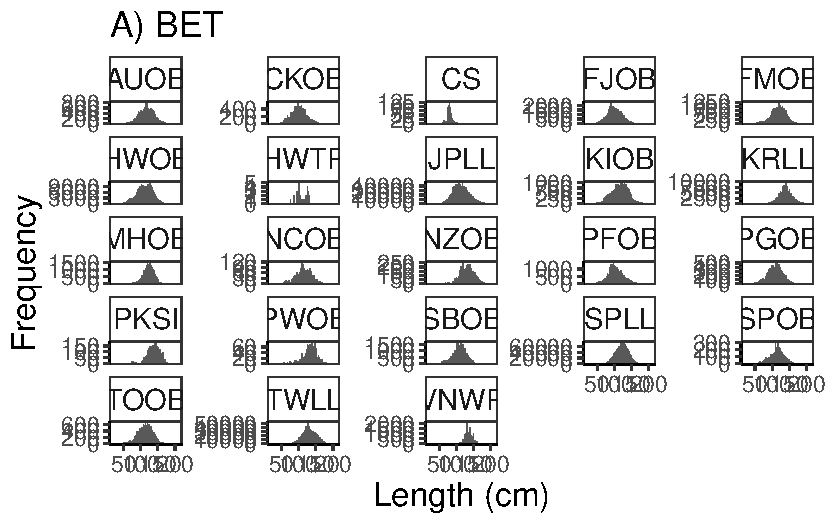
\includegraphics{length_data_explore_files/figure-pdf/raw_len_by_orig-1.pdf}

}

\caption{Raw length frequency data by sampling program. A) BET, B) YFT.}

\end{figure}

\begin{figure}

{\centering 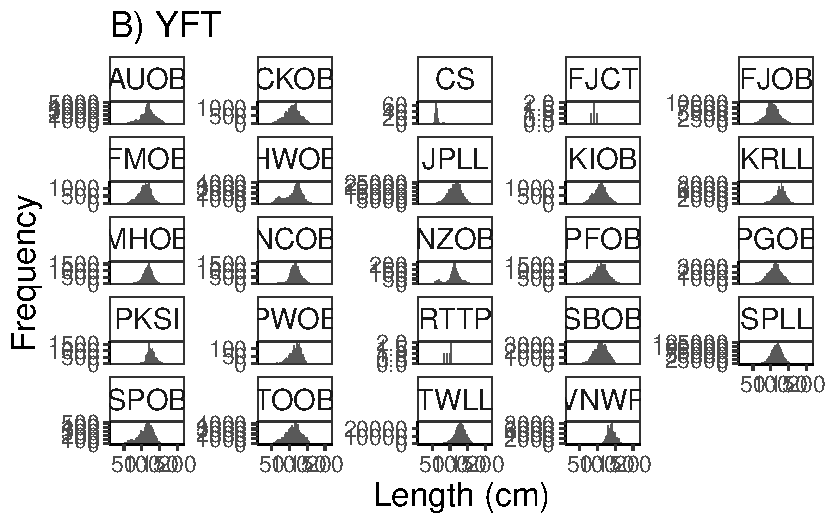
\includegraphics{length_data_explore_files/figure-pdf/raw_len_by_orig-2.pdf}

}

\caption{Raw length frequency data by sampling program. A) BET, B) YFT.}

\end{figure}

\begin{figure}

{\centering 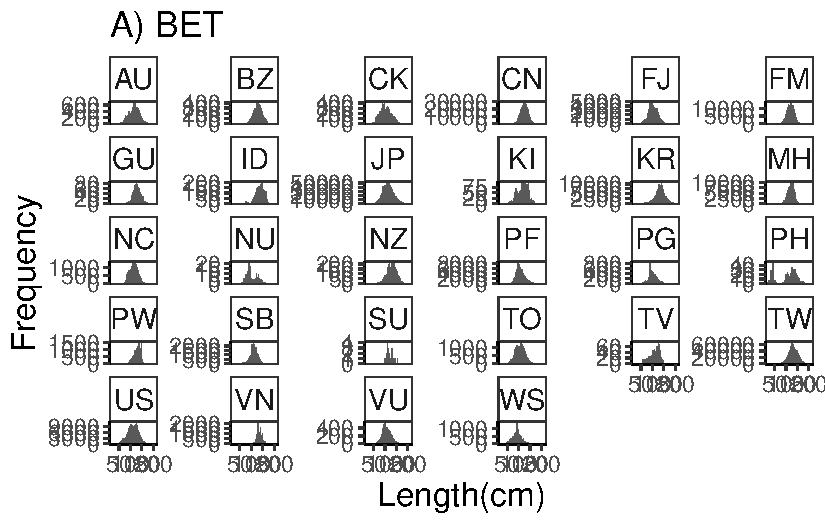
\includegraphics{length_data_explore_files/figure-pdf/raw_len_by_flag-1.pdf}

}

\caption{Raw length frequency data by flag. A) BET, B) YFT.}

\end{figure}

\begin{figure}

{\centering 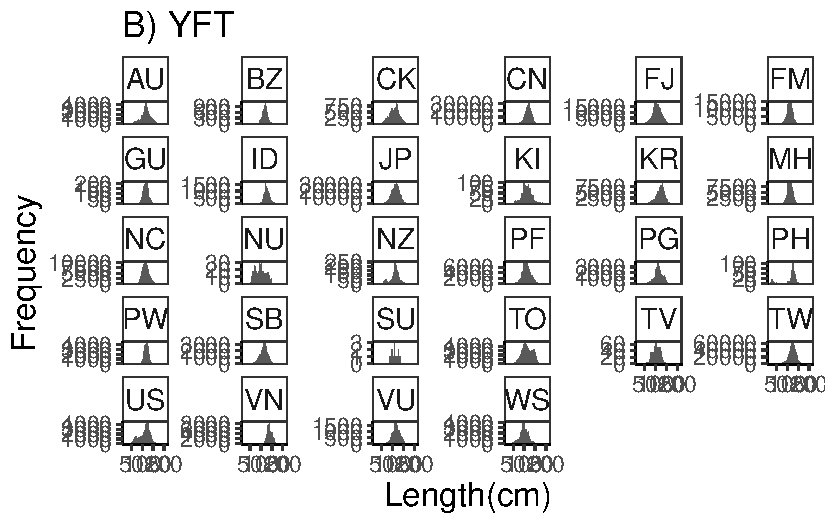
\includegraphics{length_data_explore_files/figure-pdf/raw_len_by_flag-2.pdf}

}

\caption{Raw length frequency data by flag. A) BET, B) YFT.}

\end{figure}

\begin{figure}

{\centering 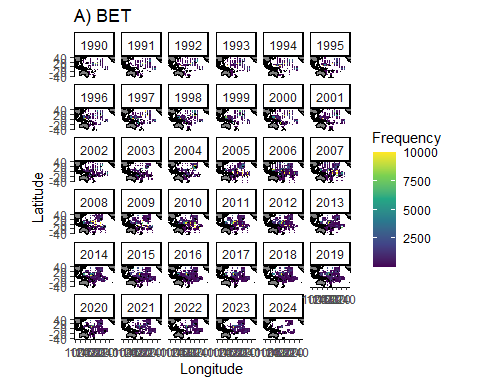
\includegraphics{length_data_explore_files/figure-pdf/raw_len_by_area-1.pdf}

}

\caption{Raw length frequency data map by year. A) BET, B) YFT.}

\end{figure}

\begin{figure}

{\centering 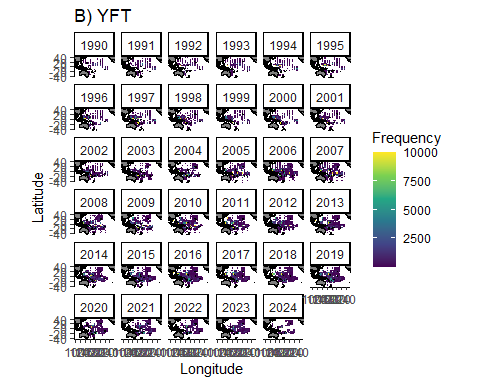
\includegraphics{length_data_explore_files/figure-pdf/raw_len_by_area-2.pdf}

}

\caption{Raw length frequency data map by year. A) BET, B) YFT.}

\end{figure}

\begin{figure}

{\centering 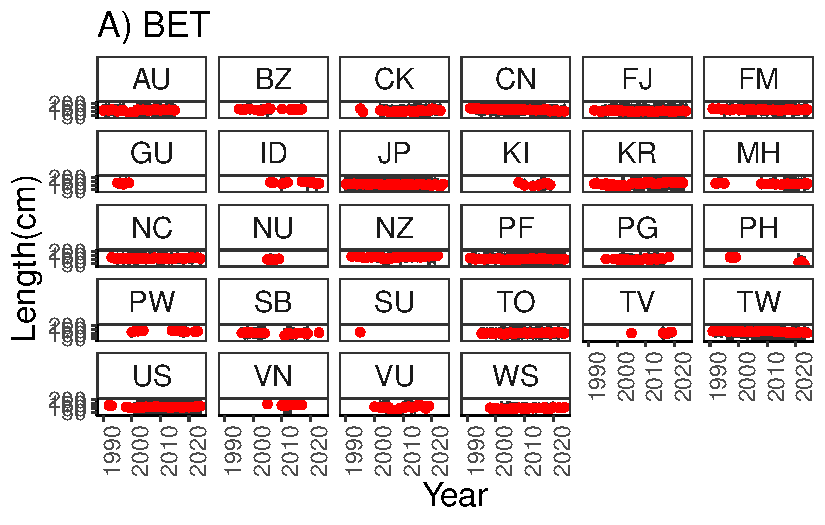
\includegraphics{length_data_explore_files/figure-pdf/yr_flag_violin-1.pdf}

}

\caption{Violin plots of length frequncies by year and flag. A) BET, B)
YFT.}

\end{figure}

\begin{figure}

{\centering 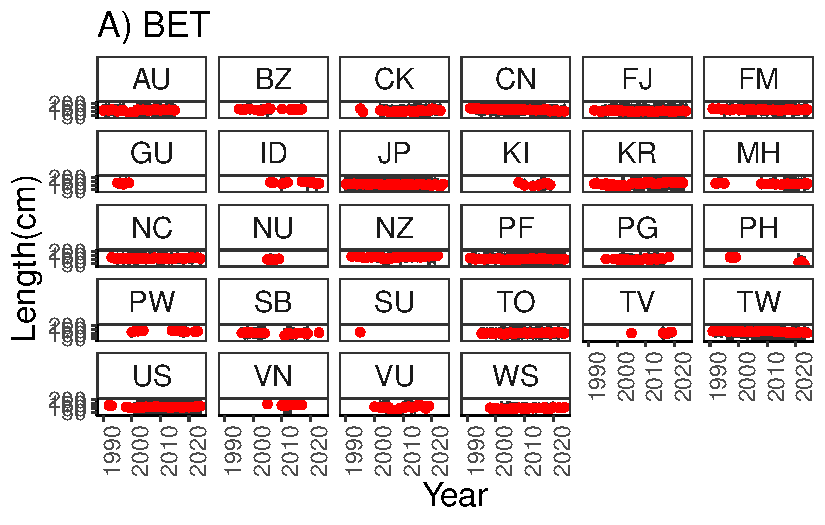
\includegraphics{length_data_explore_files/figure-pdf/yr_flag_violin-2.pdf}

}

\caption{Violin plots of length frequncies by year and flag. A) BET, B)
YFT.}

\end{figure}

\begin{figure}

{\centering 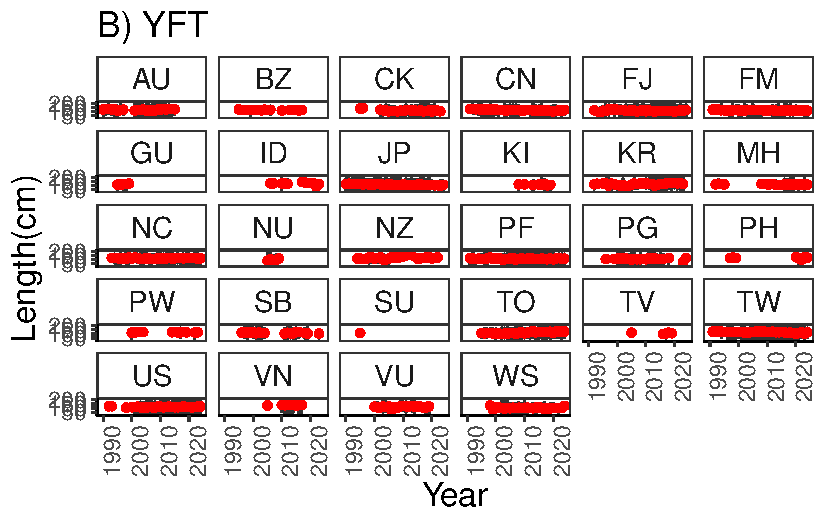
\includegraphics{length_data_explore_files/figure-pdf/yr_flag_violin-3.pdf}

}

\caption{Violin plots of length frequncies by year and flag. A) BET, B)
YFT.}

\end{figure}



\end{document}
